\chapter{Sistema di autenticazione}
Il meccanismo di autenticazione è la procedura per verificare che un determinato dispositivo
sia abilitato a connettersi alla rete.
Questo procedimento avviene tramite l'\gls{aka}, procedimento in cui
il \textit{core network} abilita un dispositivo a connettersi, e come vedremo, dal 3G anche viceversa (autenticazione mutua).\\
In questo capitolo verranno trattati le procedure di autenticazione\cite{identifications} per le generazioni dal 2G al 5G, il 1G è stato escluso 
poiché ha un funzionamento completamente analogico.

\clearpage

\section{2G}
Il sistema di autenticazione di seconda generazione utilizza principalmente due codici univoci della \gls{sim} e del \gls{ms}:
\begin{itemize}
    \item \gls{imsi} ovvero un codice identificatvo della \gls{sim}
    \item \gls{imei} ovvero un codice identificativo del \gls{ms}
\end{itemize}
Questi due codici saranno necessari anche per le prossime generazioni fino al 4G.\\
La procedura di autenticazione di un \gls{ms} segue questi passaggi:
\begin{enumerate}
    \item Il \gls{ms} invia l'\gls{imsi} alla \gls{bs} di riferimento che lo inoltra al \textit{core network}, questo
    avviene ogni volta che il \gls{ms} vuole connettersi al \textit{network} e non risulta già registrato presso 
    la rete di riferimento. In caso lo fosse, verrà utilizzato il \gls{tmsi}
    per preservare il suo anonimato.
    \item L'\gls{auc} cerca la chiave Ki associata all'\gls{imsi} e insieme a un numero casuale RAND genera un codice \gls{sres} che verrà
    salvato nel \gls{vlr}.
    \item Viene inviato al \gls{ms} il RAND generato.
    \item La stessa procedura viene fatta dal \gls{ms}, che genera quindi il suo \gls{sres} e lo invia al \gls{vlr}.
    \item Il \gls{vlr} confronta se l'\gls{sres} ricevuto corrisponde a quello generato dall'\gls{auc}, se corrispondono l'autenticazione risulta
    effettuata con successo.
\end{enumerate}

\begin{figure}[h]
    \centering
    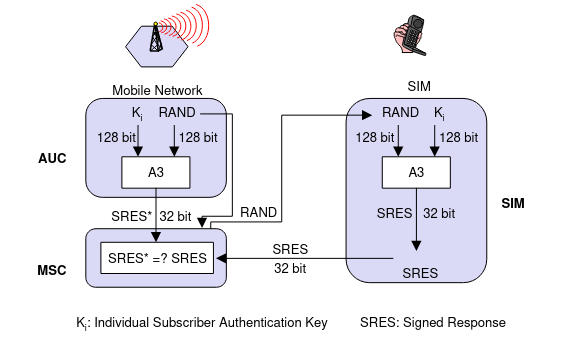
\includegraphics[width=0.7\textwidth]{images/auth-2g.png}
    \caption{Autenticazione nelle reti 2G}
\end{figure}

\clearpage

\section{3G-4G}
Dato che l'autenticazione nelle reti 3G e 4G è molto simile, verranno trattate insieme in questa sezione.
L'autenticazione nell'architettura di terza e quarta generazione è molto simile a quella della seconda salvo i seguenti miglioramenti:
\begin{itemize}
    \item Viene introdotta l'autenticazione mutua per prevenire l'autenticazione a false \textit{base stations}.
    \item La lunghezza della chiave Ki viene incrementata da 64 a 128 bit.
    \item Viene implementato un flag per verificare se le comunicazioni vengono compromesse durante la trasmissione chiamato \gls{ik}.
\end{itemize}
Il procedimento di autenticazione è il seguente\cite{4g-auth}:
\begin{enumerate}
    \item Il \gls{ms} invia l'\gls{imsi} alla \gls{bs} di riferimento che lo inoltra al \textit{core network}.
    \item L'\gls{auc} cerca la chiave Ki associata all'\gls{imsi} e insieme a un numero casuale RAND genera un codice \gls{sres} che verrà
    salvato nel \gls{vlr}.
    \item Viene trovata la chiave Ki corrispondente all'\gls{imsi} dall'\gls{auc}, dopodichè viene generato un codice \gls{sres} con l'utilizzo di un numero randomico RAND.
    Inoltre, viene generato un codice \gls{autn} per permettere al MS di autenticare il \textit{network}.
    \item Viene inviato al \gls{ms} il RAND e \gls{autn}.
    \item Il \gls{ms} autentica il \textit{network} confrontando il valore di \gls{autn} ricevuto. Se il \textit{network} è valido, prosegue con la generazione del \gls{sres}.
    \item Il \gls{vlr} confronta se il SRES ricevuto corrisponde a quello generato dall'\gls{auc}, se corrispondono l'autenticazione risulta
    effettuata con successo e viene generato,salvato e inviato il \gls{tmsi}.
\end{enumerate}
\begin{figure}[h]
    \centering
    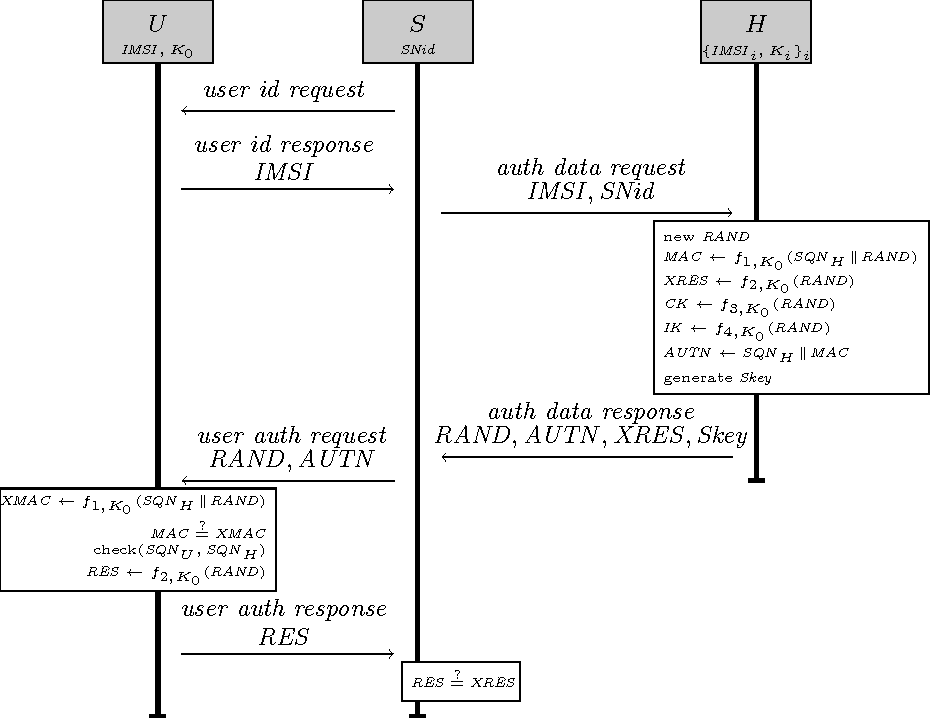
\includegraphics[width=0.7\textwidth]{images/auth-3g.png}
    \caption{Autenticazione nelle reti 3G-4G}
\end{figure}

\clearpage

\section{5G}
L'autenticazione della generazione 5G è molto diversa dalle precedenti poichè, come illustrato nella sezione 3.5, l'architettura è completamente rivista diventando una ramificazione di microservizi.
Sono definiti tre protocolli di autenticazione:
\begin{itemize}
    \item 5G-AKA: 5G-\textit{Authentication and Key Management}
    \item EAP-AKA: \textit{Extensible Authentication Protocol – Authentication and Key Management}
    \item EAP-TLS: \textit{Extensible Authentication Protocol – Transport Layer Security}
\end{itemize}
Rispetto alle generazioni precedenti ci sono stati i seguenti miglioramenti di sicurezza\cite{5g-vs-4g}:
\begin{itemize}
    \item L'\gls{imsi} non viene mai comunicato in chiaro ma sempre criptato
    \item I componenti del \textit{network} coinvolti sono dei servizi
\end{itemize}
L'autenticazione è fondamentalmente diviso in due parti: La prima è l'inizializzazione dell'autenticazione e la scelta del metodo di autenticazione.
La seconda è invece l'autenticazione mutua come avviene nelle generazioni precedenti.
Lo schema di autenticazione è il seguente\cite{5g-auth}:
\begin{enumerate}
    \item Il \gls{ms} invia il \gls{suci} o 5G-GUTI alla \gls{bs} di riferimento che lo inoltra al \gls{amf}/\gls{seaf},
    il \gls{guti} è un identificativo temporaneo simile al \gls{tmsi} delle generazioni precedenti, invece il \gls{suci} è un identificatore criptato
    permanente.
    \item il \gls{seaf} manda l'identificatore del dispositivo (\gls{suci} o 5G-GUTI) e il \gls{snn} all'\gls{ausf}.
    Il \gls{snn} è una concatenazione di codici identificativi di servizi e il codice identificativo del \textit{serving network}. Serve per capire 
    a quale \textit{slice} vuole connettersi il dispositivo.
    \item L'\gls{ausf} controlla che la richiesta dal \gls{seaf} sia autorizzata a utilizzare il \gls{snn}, in caso non lo fosse risponde con un 
    apposito messaggio di errore.
    \item L'gls{ausf} reperisce la chiave associata all'identificativo nell'archivio \gls{udm} e genera il rispettivo \gls{sres} con un numero randomico RAND.
    \item Viene inviato all'\gls{ms} il RAND e \gls{autn} (per l'autenticazione mutua).
    \item Il \gls{ms} procede con la creazione del \gls{sres} e lo invia al \gls{seaf}.
    \item Il \gls{seaf} inoltra il \gls{sres} all'\gls{ausf} che si occupa di controllare se corrispondono e in caso confermare l'autenticazione.
\end{enumerate}
\begin{figure}[h]
    \centering
    \includegraphics[width=1\textwidth]{images/auth-5g.png}
    \caption{Autenticazione nelle reti 5G}
\end{figure}